\section{Rear: Rear Exocentric Augmented Reality}
\label{sec:rear}

\subsection{How it works}
In this chapter we briefly describe how all the exocentric vision
is implemented, along with its business logic. In order to achieve
this, we will occasionally refer to the class diagram shown in figure
\ref{fig:class_diagram}.
%
\begin{figure}[!h]
  \begin{center}
    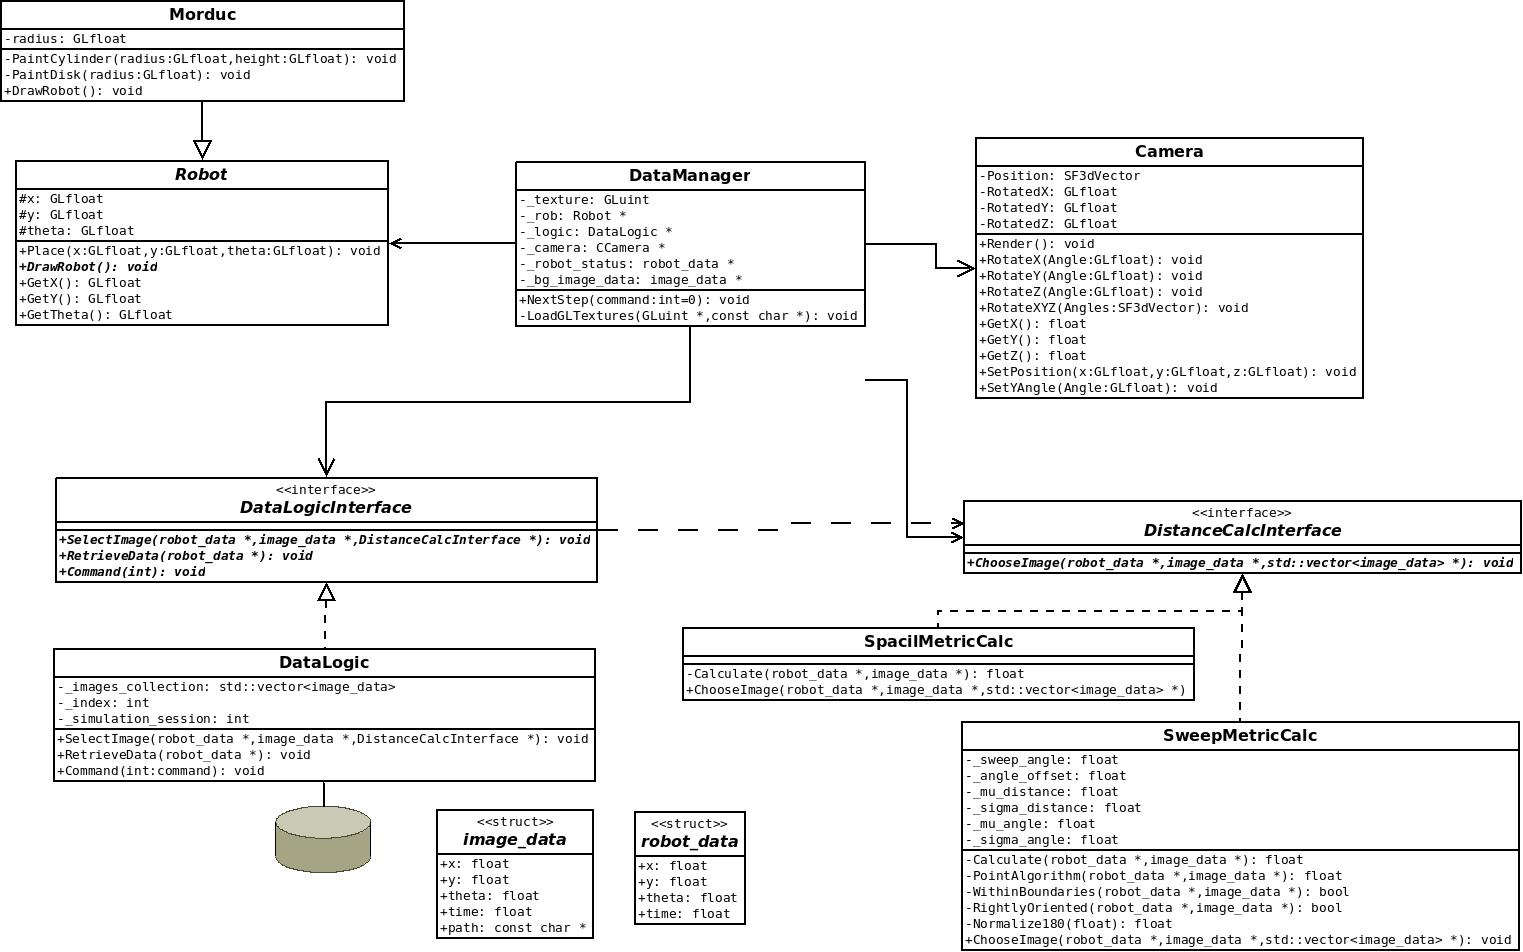
\includegraphics[width=400pt]{img/class_diagram.jpeg}  %robot pic
    \caption{Application class diagram}
    \label{fig:class_diagram}
  \end{center}
\end{figure}
%
The overall schema can be resumed by the following diagram (see figure
\ref{fig:overall_diagram}). User sends a command to the exocentric vision
application, in order to guide the robot through the remote environment.
The exocentric vision application forwards the command to the robot or the
simulator (paragraph \ref{sec:simulator}) and waits for the response.
The latter includes the new robot position and the new egocentric camera images.
%

%
All the egocentric camera images retrieved are stored in a data set and coupled
with robot coordinates and orientation at the moment when they were shot. Going
on with the application a large collection of egocentric images will be gathered.
%
\begin{figure}[!h]
  \begin{center}
    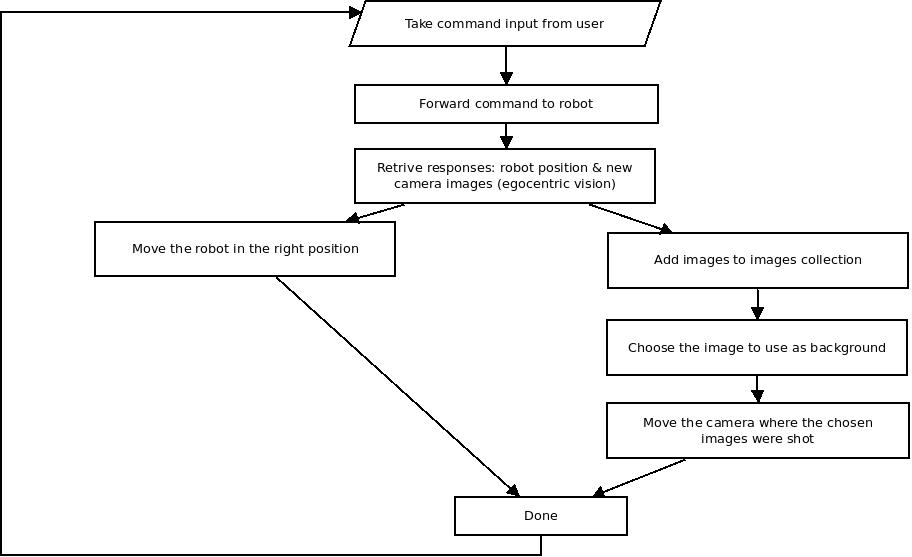
\includegraphics[width=400pt]{img/overall_diagram.jpeg}  %robot pic
    \caption{Application flowchart}
    \label{fig:overall_diagram}
  \end{center}
\end{figure}
%
After retrieving response from robot, the exocentric vision application moves the
robot in the openGL world (according to the robot coordinates read) and adds the
images received to the images collection. Later on, the application has to choose
the proper image (among those collected in the set) to use as texture (i.e. background)
in OpenGL and implement the exocentric vision.
%

%
Since every image owns its data about position and orientation when shot, we can
move and point the camera object to obtain the right visual of the external world.
Wherever the robot is situated, we will be able to watch it from the right point of view,
depending on the texture image chosen.
%

%
All the process explained above is lacking of one part: how to choose the background image,
knowing the actual robot position and orientation. If we decided to choose the closest image
to the robot we would always show the egocentric vision, because the algorithm would select
always the image with the same position and orientation of the robot. The distance between
the robot and the selected images would be equal to zero, which is doubtless the minimum possible
value.
%

%
The algorithms to take the right image in exocentric vision can be various. Each one has its own
advantages and disadvantages, we will chose the one able to guarantee the best trade-off.

\subsection{How to choose the right background image}
There are many ways of choosing the background image among the collected ones. This unique
block, entitled "choose K" in diagram \ref{fig:overall_diagram}, can be thought of as a
black box, with the robot position and orientation data as input and the background image
(or better, its path) as output.
%

%
To make easier the definition and the deployment of a new algorithm, the interface
\texttt{DistanceCalcInterface} has been declared, with only one pure virtual method named
\texttt{Calculate}. Every new algorithm able to choose a background image has to be defined
within the \texttt{Calculate} function.
\texttt{Calculate} return a float value, that is a score value; the parameters taken are a
single image and the robot data. When the robot changes its position or orientation, the
framework built computes the "Calculate" function for every image, with the new robot values.
Every image is therefore coupled with a score, and the one with minimum associated value will
be chosen.
%

%
All you need to run a different algorithm is to instance the right object implementing the
\texttt{DistanceCalcInterface} and link it with the \texttt{DataManager}, who will automatically
use the custom function to evaluate the score for every stored image. As written before, the
one with the lowest score will be rendered as background texture.
%

%
For instance, if the target is to select the image shoot closest to the actual robot position,
the returned score will be the euclidean distance between the image and robot itself. In this way
the minimum score will be associated with the closest image.
The algorithm described above is implemented within the \texttt{Calculate} function of the
\texttt{SpacialMetricCalc} class (see class diagram \ref{fig:class_diagram}). Another class, named
\texttt{SweepMetricClass}, implements the \texttt{DistanceCalcInterface}, but it defines a totally
different and more complex algorithm. Chapter \ref{subsec:sweep_angle_algorithm} will explain
it in detail.

\subsection{The "sweep angle" algorithm}
\label{subsec:sweep_angle_algorithm}
The "sweep angle" algorithm allows to choose the better background image, in order to implement
the exocentric vision.
%
\begin{figure}[!h]
  \begin{center}
    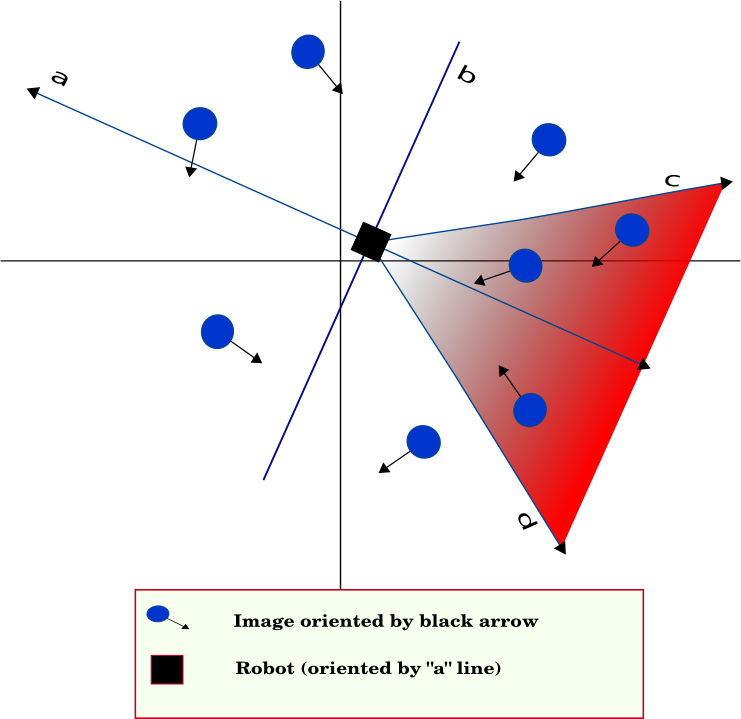
\includegraphics[width=400pt]{img/half_plan_finding.png} 
    \caption{Sweep Angle Algorithm}
    \label{fig:half_plan_finding}
  \end{center}
\end{figure}
%
All the explanation will refer to image \ref{fig:half_plan_finding}. In the latter, the black
square represents the robot, with its orientation indicated by the arrow "a", starting from the
square.
%

%
The several blue circles represent instead the previous shoot images. The orientation of each
image (i.e. the orientation of the robot when they were shoot) is shown by an arrow starting from
each circle.
%

%
We will refer to the line perpendicular to the half line "a" as "b". By rotating clockwise and
counterclockwise the "a" line in the robot centre with a predefined angle (named "sweep angle")
we will obtain the "c" and "d" lines. These define a new portion of the plane (coloured with fading red),
named the "sweep area".
%

%
Since we want to control the robot from the rear position, the sought image will be included within
this area: all the other ones will be discarded. Even tough this method allows us to exclude many
images, the selection is certainly not over.
%

%
First of all, we have to discard all the images with an orientation angle that differs too much from the
robot orientation angle. If the difference between the two angles is greater than a specified threshold,
the image can not be chosen as background, because the latter does not include the robot from its point
of view. For instance, if the difference angle between the robot and the image orientation is 180 degrees,
it means that robot and camera are oriented in opposite way, therefore the camera can not see the robot
itself.
%

%
After excluding the badly oriented images, we proceed with the score assignment. The latter is obtained by
the sum of two factors. The first takes in account the image angle orientation: the more the image orientation
angle is close to the robot orientation angle, the more the score is high.
%

%
The function to evaluate the score from the difference between the two angles is a Gaussian function centre
in zero. The return value will be therefore always a positive number.
%

%
The use of a Gaussian function allows to obtain different values even for two very close angle difference
(Gaussian is a injective function), regardless of the assigned variance. Moreover, it is defined for all real
numbers.
In this way is always possible to discern the best angle difference, by choosing the highest value returned by
the function.
%

%
Finally, we have to take in account the euclidean distance between the image and the robot. If the distance is
zero, we are examining the egocentric image. On one side, the images too close to the robot will be coupled
with a low score, because they are too similar to the egocentric one. On the other side, the images too far
from the robot will be coupled again with a low score, because they would show the robot too distance to
teleguide it properly.
%

%
The preferable image would distance from the robot a predefined quantity, specified by the user. This value
indicate us where to centre another Gaussian function, in order to obtain the score from the distance between
image and robot. The more the image is close to the preferred distance, the more the score assigned will be high.
%

%
The reasons that justifies the use of the Gaussian function are the same previously explained for the angle
difference. The values obtained from the two Gaussian functions, after adding them, form the global score.
%

%
To summarize the method above illustrated (illustrated in figure \ref{fig:sweep_angle_diagram}), we coupled
every image with a score: the one with the maximum value will be chosen and put as background. If the image is
not included in the sweep area (defined by a sweep angle and therefore by the "c" and "d" line) it has to be
discarded. The score assigned will be -2.
%
\begin{figure}[!h]
  \begin{center}
    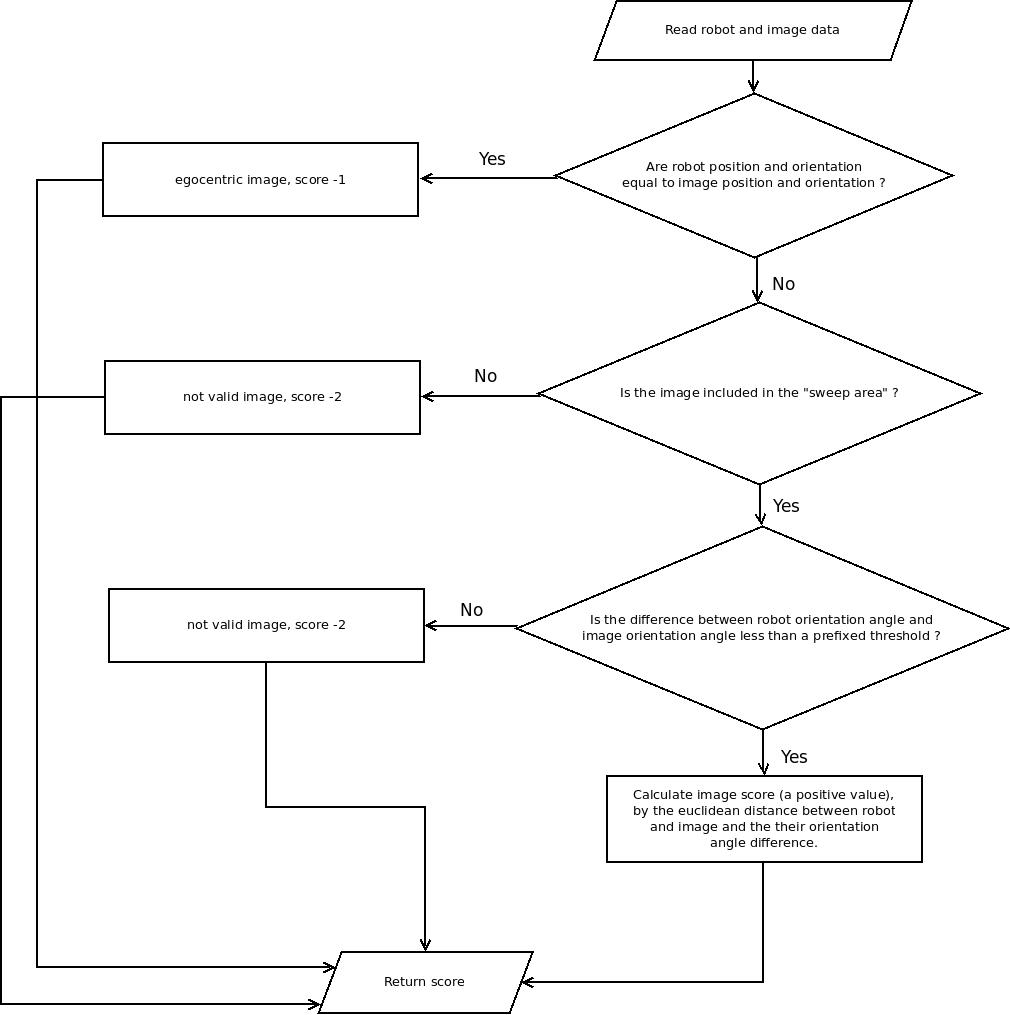
\includegraphics[width=400pt]{img/sweep_angle_diagram.jpeg} 
    \caption{Sweep angle diagram}
    \label{fig:sweep_angle_diagram}
  \end{center}
\end{figure}

%
The images situated within the sweep area, but with an orientation angle that differs too much from the robot
orientation angle, have to be discarded as the previous one: the score assigned will be -2 again.
If the image position and orientation coincide with robot position and orientation, the image represents the
egocentric vision. We remember that in our set there will always be the egocentric image, and that this will be
choose as background when no other image for exocentric vision are available. The score coupled with the egocentric 
vision will be -1.
%

%
Finally, all the other images - if present - are coupled with a positive number, because obtained by the sum of
values calculated with Gaussian functions. The most high score indicate the better image to chose as background;
if there are no preferable images, the image with -1 (i.e. the egocentric image) will be chosen.
%

%
Because the DataLogic is designed to choose the image with the minimum score and not with maximum, all we have to
do is multiply every score for -1 before returning it: in this way we convert a maximum research in a minimum one.
%

\subsection{The Robot class}
The robot class, present in Filippo Privitera's simulator 
\cite{privitera}, has been simplified and then introduced in
exocentric vision control code. In this chapter we will 
exam the main differences.
%

%
Both classes represent the 3morduc robot in openGL world. 
This means that the robot class offers, among others, a
method with the purpose of drawing itself, called by the 
OpenGL framework when it is necessary. The operation of 
drawing is completed thanks to other two methods, able 
to draw the elementary part of the robot - e.g. cylinders and disks.
%

%
There are not considerable different between the tho 
drawing method implantation. The main one is that in the 
new method, before starting drawing, the model-view matrix 
is copied in order to restore it at the end of the process. 
In these way we do not affect the model-view matrix status 
by drawing the robot.
%

%
The robot class, after the refactoring process, loses many 
of its public attributes and methods, so in the
exocentric vision control it is much more simple than the 
original one. First of all, the new class does not contain either
attributes to store the actual speed vector component, or 
a chronometer object to count the time, or information about wheels
encoder. This information was stored in the simulator robot 
class to calculate the position of the robot after a movement,
but since we retrieve the position directly from the simulator 
these fields are now useless. 
%

%
The unique attribute (changed from public to private, in 
the new version) which survives the refactory - along with the
triple values indicating coordinate on x axis, coordinate on 
y axis and rotation - is named \texttt{radius}. \texttt{radius}
is a float attribute, which stores the value of the radius for the 
tree cylinders which make up the robot. See figure
\ref{fig:3morduc_opengl} for a better understanding.
%
\begin{figure}[!h]
  \begin{center}
    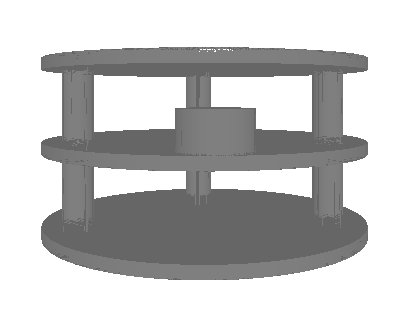
\includegraphics[width=200pt]{img/3morduc_opengl.png}  %robot pic
    \caption{The 3morduc robotic platform drawn in OpenGL}
    \label{fig:3morduc_opengl}
  \end{center}
\end{figure}
%
The default \texttt{radius} value is 4, but it can be 
customised by the user: by increasing it the robot will be 
displayed larger and larger on the screen, and viceversa.
%

%
All the attributes are private in the new robot class, 
so a method to get each one value is declared. 
%

%
Most of the previous public methods have been removed too. 
The constructor method, for instance, is present with one
only definition and default parameters, instead of declaring 
it twice (with parameter and without). The methods to set
linear and angular velocity are not present anymore, for 
the reason explained above; those to increment the collisions 
number are actually disabled because, at this development 
stage, the exocentric vision control does not face the collision 
problem. Anyway, it is supposed to cope with collision in 
the future version.
%

%
Besides, the method used by Privitera's simulator to read 
the robot initial position from file has been removed, since 
for the exocentric vision system robot always starts from 
fixed coordinates and rotation.
%

%
Finally, the method named with the signature 
\texttt{void move()} has been changed in \texttt{void Place(float x, float y, float theta)}
in order to set the x and y coordinate and the rotation of the robot. 
We remind that in the previous version these attributes
were public, so there were no need to pass them as parameters function.

\subsection{The Camera class}
First of all, there is no thing like a camera in OpenGL, therefore we have to
simulate one.
%

%
A camera object allows to move and rotate the user point of view and robot
object independently, avoiding that one interferes the other. For the exocentric
vision application this is a basic feature, because robot can be placed
everywhere in OpenGL world regardless of the camera position, and viceversa.
%

%
The camera object implementation has been suggested by \cite{opengl:camera}.
It provides some elementary commands implemented by means of mathematical matrix
operations, to move the camera or rotate it along one axis.
